%!TEX root = ../guide.tex

\section{Usage Scenarios}
\label{sec:3}

This section introduces how to use the framework for common usage scenarios. The examples are at the high level, no code is provided. If you want to refer to concrete examples in code, please refer to the package \emph{ch.epfl.ts.example} or check it out on \href{https://github.com/merlinND/TradingSimulation/tree/master/ts/src/main/scala/ch/epfl/ts/example}{Github}.

\subsection{Bitcoin Trading}

In this example, we demonstrate how to use the framework to experiment Bitcoin trading with the \emph{MovingAverageTrader} on live market data. The component graph of this application is as follows:

\noindent
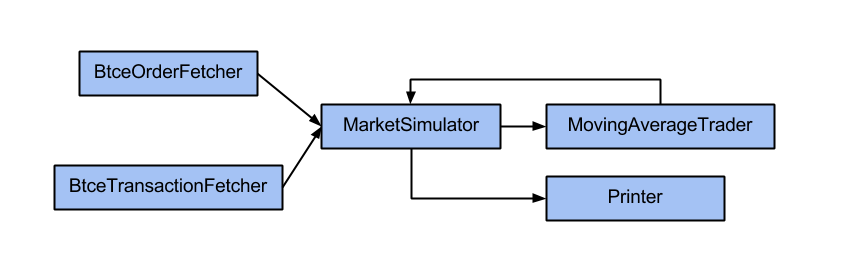
\includegraphics[width=\textwidth]{img/examples/btce}

The BTC-E fetchers get orders and transactions from \url{http://btc-e.com}, feed them to the market simulator. The market simulator generates transactions based on the bid and ask orders from the trader. The trader sends bid or ask orders to the market simulator based on the transactions received from the market simulator. The printer prints information about the market in the console.

\subsection{Forex Trading}

In this example, we demonstrate how to use the framework to experiment Forex trading with the \emph{MovingAverageTrader} on live Forex data. The component graph of this application is as follows:

\noindent
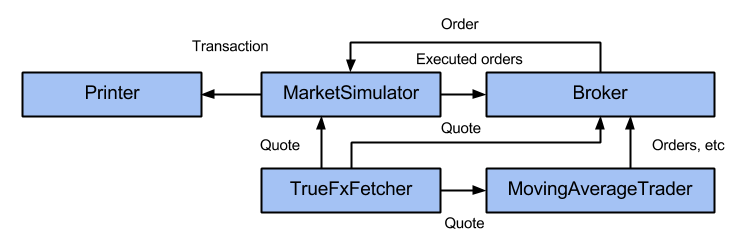
\includegraphics[width=\textwidth]{img/examples/forex-live}

In the component graph above, the fetcher gets live quotes data from \url{http://webrates.truefx.com}, and feeds them into the market simulator, trader and broker.

The trader makes sell and buy decisions based on the quotes received from the fetcher, and send them to the broker.

The broker receives orders from the trader, and forward them into the market simulator on behalf of the trader. Note that the usage of broker is optional, it's used here only for illustrating purpose.

The market simulator generates transactions based on the orders received from brokers, and sends the transaction result back to the broker.


\subsection{Evaluating the Performance of Traders}

This example demonstrates how to evaluate the performance of a trader. For this purpose, we have to use the component \emph{Evaluator}. The \emph{Evaluator} encapsulates a trader component -- that means if you want to connect an upstream component to the trader, you can connect it to the \emph{Evaluator}. And if you want to connect the trader to a downstream component, you connect the \emph{Evaluator} to the downstream component. The wirings inside \emph{Evaluator} will ensure that everything works correctly just like you wire the two components separately.

The component graph is as follows:

\noindent
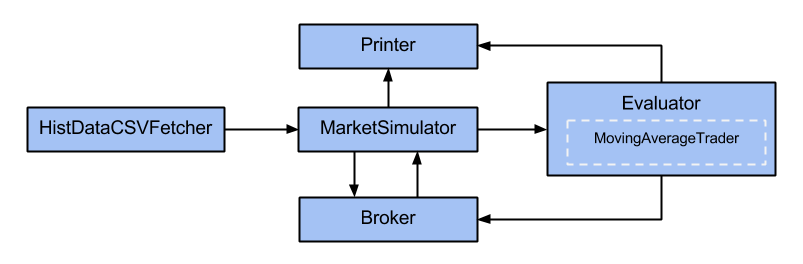
\includegraphics[width=\textwidth]{img/examples/evaluation}

As it's show in the graph above, the evaluator encapsulates an instance of the \emph{MovingAverageTrader}. They should be considered as a single component, instead of two. It receives transaction and quote data from the market simulator. It sends evaluation report to the printer, and orders to the broker.

The market simulator receives orders from the broker and quotes from the fetcher. It sends the transaction result back to the broker.

The fetcher reads history quotes from file system and sends them to the market simulator. Which fetcher or dataset to use for the evaluation is up to the designer of the experiment.

If you're interested in a code example, you can checkout out at \href{https://github.com/merlinND/TradingSimulation/blob/master/ts/src/main/scala/ch/epfl/ts/evaluation/EvaluationRunner.scala}{Github}.

\subsection{Full Market Simulation}

TradingSimulation provides the possibility to experiment with full market simulation. In ideal full market simulation, all market data are generated from the transactions of traders, it's a closed world. However, there's a problem on how to start the market initially. The approach we choose is to seed the market with history data, and cut the data source once the market gets activated. The two different modes of the market require different market rules in order for the market to function normally.

Due to this special requirement to disconnect components and change market rules at runtime, we defined a special market simulator \emph{HybridMarketSimulator} for full market simulation. The component graph is as follows:

\noindent
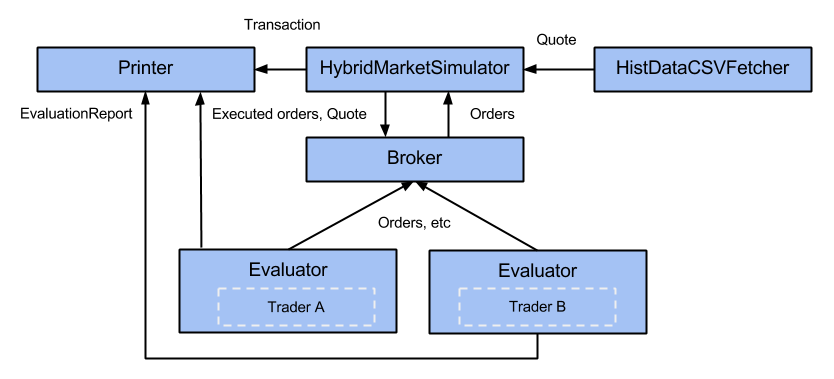
\includegraphics[width=\textwidth]{img/examples/full-simulation}

In the graph above, there're only two traders, but you can add as many traders as you need. The traders are encapsulated in evaluators, so that the printer can print the performance of traders in the console.

In the full simulation, it's important to cut off the data source once the market gets activated. This can be achieved using following code snippet:

\begin{lstlisting}[language=Scala]
  val timer = new Timer()
  class StopFetcher extends java.util.TimerTask {
    def run() {
      quoteFetcher.ar ! StopSignal
      market.ar ! 'ChangeMarketRules
    }
  }
  timer.schedule(new StopFetcher, delay)
\end{lstlisting}

For a complete example of full market simulation in code, please refer to the example \emph{FullMarketSimulation} in the code base. You can check it out at \href{https://github.com/merlinND/TradingSimulation/blob/master/ts/src/main/scala/ch/epfl/ts/example/FullMarketSimulation.scala}{Github}.
